\documentclass[border=1pt]{standalone}
% Shared preamble for standalone figures in this directory.
% Compile with XeLaTeX from 讲义/figs, or via the figures target.
\usepackage{ctex}
\usepackage{amsmath}
\usepackage{amssymb}
\usepackage{bm}
\usepackage{mathtools}
\usepackage{tikz}
\renewcommand{\vec}[1]{\boldsymbol{#1}}
\newcommand{\cC}{\mathcal{C}}
\newcommand{\cD}{\mathcal{D}}
\newcommand{\R}{\mathbf{R}}
\usetikzlibrary{
    arrows.meta,
    calc,
    decorations.markings,
    angles,
    quotes,
    positioning,
    patterns,
    shapes.geometric
}

\begin{document}
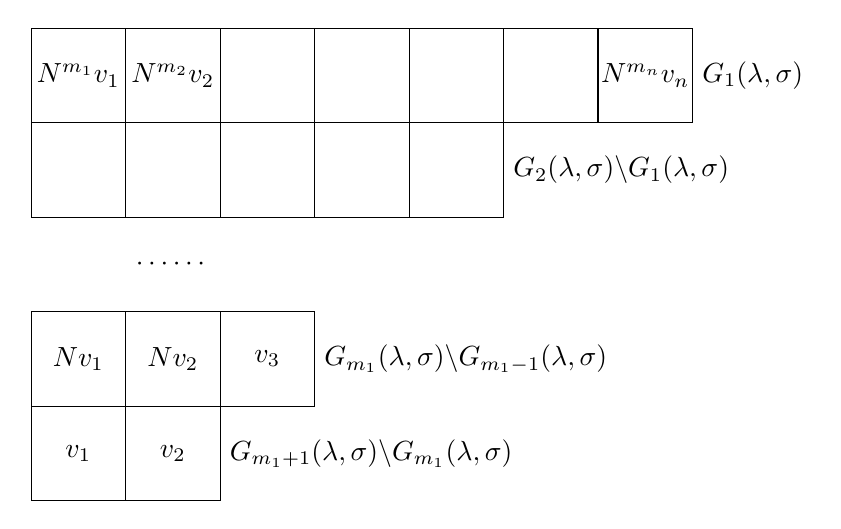
\begin{tikzpicture}[scale=1.2]
    \foreach[count=\i] \len in {7, 7, 5, 3, 3, 2}
    \draw (0, -\i+1) -- (\len, -\i+1);

    \foreach \i in {0, 1, 2}
    \draw (\i, -3) -- (\i, -5);

    \draw (3, -3) -- (3, -4);

    \foreach \i in {0,...,5}
    \draw (\i, 0) -- (\i, -2);

    \foreach \i in {6, 7}
    \draw (\i, 0) -- (\i, -1);

    \foreach \i in {1, 2} {
    \node at (\i-.5, -4.5) {$v_{\i}$};
    \node at (\i-.5, -.5) {$N^{m_{\i}}v_{\i}$};
    }
    \foreach \i in {1, 2}
    \node at (\i-.5, -3.5) {$Nv_{\i}$};

    \node at (3-.5, -3.5) {$v_{3}$};
    \node at (6.5, -.5) {$N^{m_n}v_n$};
    \node at (1.5, -2.5) {$\cdots\cdots$};

    \node[anchor=west] at (7, -.5) {$G_1(\lambda,\sigma)$};
    \node[anchor=west] at (5, -1.5) {$G_2(\lambda,\sigma) \backslash G_1(\lambda,\sigma)$};
    \node[anchor=west] at (3, -3.5) {$G_{m_1}(\lambda,\sigma) \backslash G_{m_1-1}(\lambda,\sigma)$};
    \node[anchor=west] at (2, -4.5) {$G_{m_1+1}(\lambda,\sigma) \backslash G_{m_1}(\lambda,\sigma)$};
\end{tikzpicture}

\end{document}
